\documentclass[border=20pt]{standalone}
\renewcommand\familydefault{\sfdefault} % Default family: serif
\usepackage{tikz}
\usetikzlibrary{calc}
\usetikzlibrary{shapes.geometric}
\usetikzlibrary{arrows.meta,arrows}
\usetikzlibrary{positioning}
\tikzset{
  initial/.style={circle, fill},
  decision/.style={diamond, black, draw},
  action/.style={rectangle, draw, rounded corners},
  arrow/.style={draw, -{Latex[length=3mm]}, thick}
  }
\begin{document}
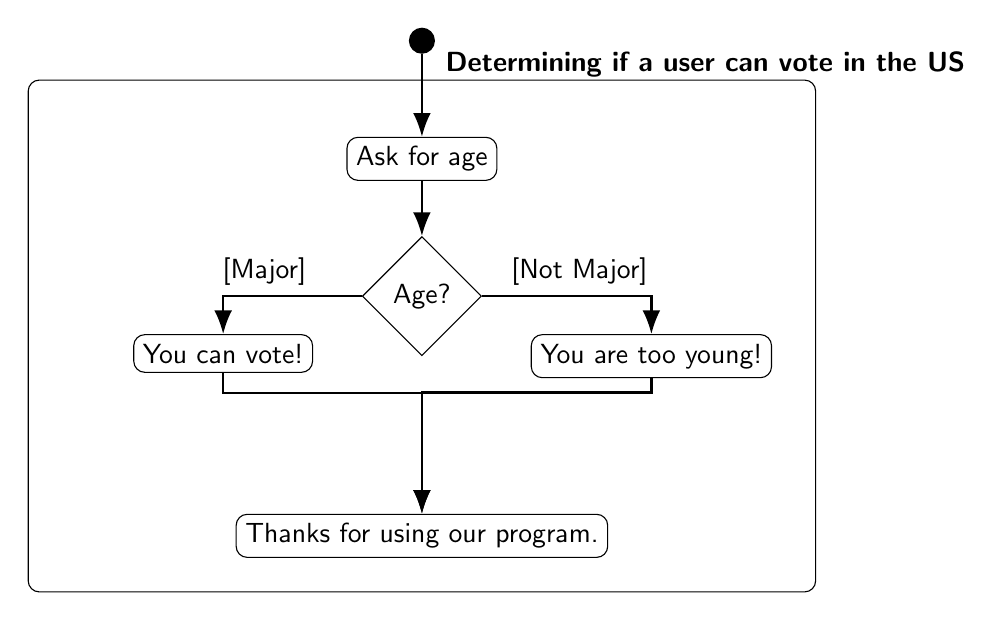
\begin{tikzpicture}[node distance=1.5cm]
	% Frame
	\draw [rounded corners] (-5,-1.5) rectangle (5, -8);
	\node (title) at (3.6, -1.3) {\textbf{Determining if a user can vote in the US}};

	% Nodes
	\node[initial] (initial) at (0,-1) {};
	\node[action, below of = initial] (ask)  {Ask for age};
	\node[decision, below = .7cm of ask] (decision1) {Age?};
	\node[action, below left = .1cm and 1cm of decision1] (major) {You can vote!};
	\node[action, below right = .1cm and 1cm of decision1] (young) {You are too young!};
	\node[action, below = 2cm of decision1] (exit) {Thanks for using our program.};

	% Arrow
	\draw [arrow] (initial) -- (ask);
	\draw [arrow] (ask) -- (decision1);
	\draw [arrow] (decision1) -- node[above, pos=1pt]{[Major]} ++(-2cm, 0) -| (major);
	\draw [arrow] (decision1) -- node[above, pos=1pt]{[Not Major]} ++(2cm, 0) -| (young);
	% Arrows to exit
%	\draw [arrow] (decision1) -- (exit);
	\draw [arrow] (major) -- ++(0cm, -.5cm) -| (exit);
	\draw [arrow] (young) -- ++(0cm, -.46cm) -| (exit);

\end{tikzpicture}
\end{document}

